\documentclass[11pt]{article}
\usepackage[utf8]{inputenc}
\usepackage[left=2cm,right=2cm,top=2.5cm,bottom=2.5cm,a4paper]{geometry}
\usepackage{helvet}
\usepackage{amsmath, amssymb, amsthm}
\newtheorem{theorem}{Theorem}
\newtheorem*{theorem*}{Theorem}
\newtheorem{corollary}{Corollary}
\theoremstyle{definition}
\newtheorem{problem}{Problem}
\newtheorem{definition}{Definition}
\newtheorem{example}{Example}
\newtheorem{axiom}{Axiom}
%%%%%%%%%
\setlength{\parindent}{0pt}
%%%%%%%%%
\title{Partially Ordered Set}
\usepackage{graphicx}
\DeclareGraphicsExtensions{.pdf,.png,.jpg}
\usepackage{float}
\usepackage{hyperref}
\hypersetup{
	colorlinks,
	citecolor=black,
	filecolor=black,
	linkcolor=black ,
	urlcolor=black
}
\author{\tt \href{https://github.com/Sanya-Lee/}{Sanya-Lee}}
\begin{document}
	\maketitle
	\begin{definition}
		Let $P$ be a set and $\leq$ be a relation on $P$.
		$(P, \leq)$ is called poset(partially ordered set) if
		\begin{itemize}
			\item $\forall a \in P , a \leq a$  , \hfill (reflexive)
			\item $\forall a, b, c \in P , a \leq b \land b \leq c \implies a \leq c$  , and \hfill (transitive)
			\item $\forall a, b \in P, a \leq b \land b \leq a \implies a = b$  . \hfill (antisymmetric)
		\end{itemize}
	\end{definition}
	
	\begin{definition}
		Let $(P, \leq)$ be a poset.
		\begin{itemize}
			\item $x, y \in P$ are called comparable if $x \leq y$ or $y \leq x$. 
			Otherwise, they are called incomparable.
			\item $x < y \iff x \leq y \land x \neq y$.
			\item $x \in P$ is called maximal if $x \not\leq y$ for all $y \in P$.
			If a maximal element is unique, then it is called maximum.
			\item $y \in P$ is called minimal if $y \not\leq x$ for all $x \in P$.
			If a minimal element is unique, then it is called minimum.
		\end{itemize}
	\end{definition}
	
	\begin{example}
		$(2^{[3]}, \subseteq)$ is a poset.
		$\emptyset$ is the minimum element and $[3]$ is the maximum element.
		\begin{figure}[H]
			\begin{center}
				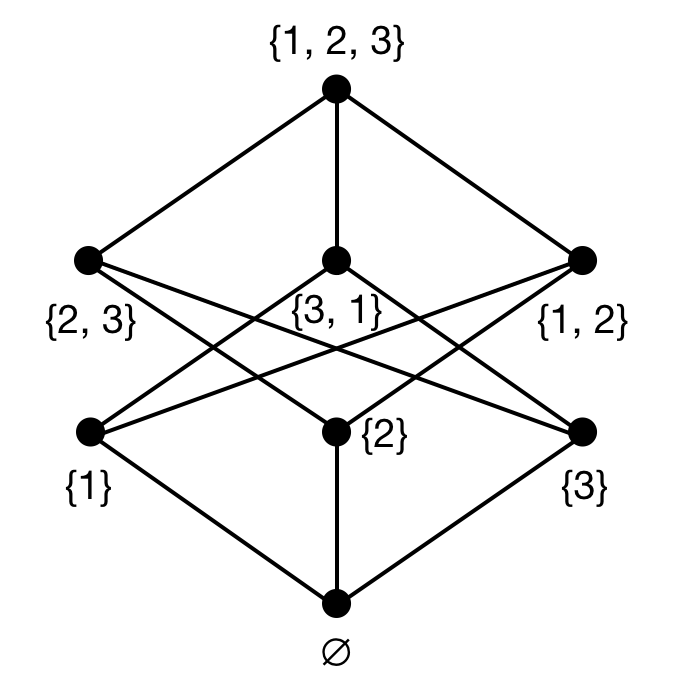
\includegraphics[scale= 0.35]{Fig00.png}
			\end{center}
		\end{figure}
	\end{example}
	
	\begin{definition}
		Let $(P, \leq)$ be a poset. 
		\begin{itemize}
			\item For $C \subseteq P$, it is called chain if any distinct two of $C$ are comparable.
			\item For $A \subseteq P$, it is called antichain if any distinct two of $A$ are incomparable.
		\end{itemize}
	\end{definition}
	
	\begin{example}
		$(\{2, 3, 4, 6, 9, 12, 13, 17\}, |)$ is a poset. \hfill($|$ : divisibility relation)
		\begin{itemize}
			\item $\{2, 6, 12\}$ is a chain.
			\item $\{4, 9, 13, 17\}$ is an antichain.
		\end{itemize}
	\end{example}
	
	\begin{theorem}
		Let $(P, \leq)$ be a poset and its longest chain has length $r$.
		Then, it can be partitioned into $r$ antichains.
	\end{theorem}
	
	\begin{proof}
		For each $x \in P$, define $l(x)$ as the length of longest chain containing $x$ as the maximum element. 
		For $m = 1, 2, \cdots , r$, define $A_i = \{ x \in P : l(x) = i \}$. 
		Then, $\{A_1, A_2, \cdots, A_r \}$ is a partition of $P$ and each $A_i(1\leq i \leq r)$ is an antichain, and it concludes our proof.
	\end{proof}

	\begin{theorem}(Dilworth's Theorem)
		Let $(P, \leq)$ be a poset and its largest antichain has size $r$. Then, it can be partitioned into $r$ chains.
	\end{theorem}

	\begin{proof}
		Use induction on $|P|$.
		
		It is clear that the theorem holds on base case.
		
		Let $a$ be a maximal element of $P$ and define $P^{\prime} = P \setminus \{a\}$.
		Define $r$ as the size of the largest antichain of $P^{\prime}$.
		Then, by induction hypothesis, $P^{\prime}$ can be partitioned into $r$ chains, say $C_1, C_2, \cdots, C_r$.
		We claim that $P$ has an antichain of size $r+1$ or $P$ can be partitioned into $r$ disjoint chains.
		Every antichain in $P^{\prime}$ of size $r$ contains exactly one element of each $C_i(1 \leq i \leq r)$.
		Define $a_i$ as maximal element of $C_i$.
		Then $A = \{a_i : i \in [r] \}$ is an antichain.
		If $A \cup \{a\}$ is an antichain, we are done.
		Suppose not.
		Then, there exists $i \in [r]$ such that $a > a_i$.
		Then, $K = \{x \in C_i : x \leq a_i \} \cup \{a\}$ is a chain of $P$.
		Since there is no antichain on $P \setminus K$ of size $r$, it can be partitioned $r-1$ chains, and it concludes our proof.
	\end{proof}
	
	\begin{example}
		$(2^{[3]}, \subseteq)$ can be partitioned into 3 chains.
		\begin{figure}[H]
			\begin{center}
				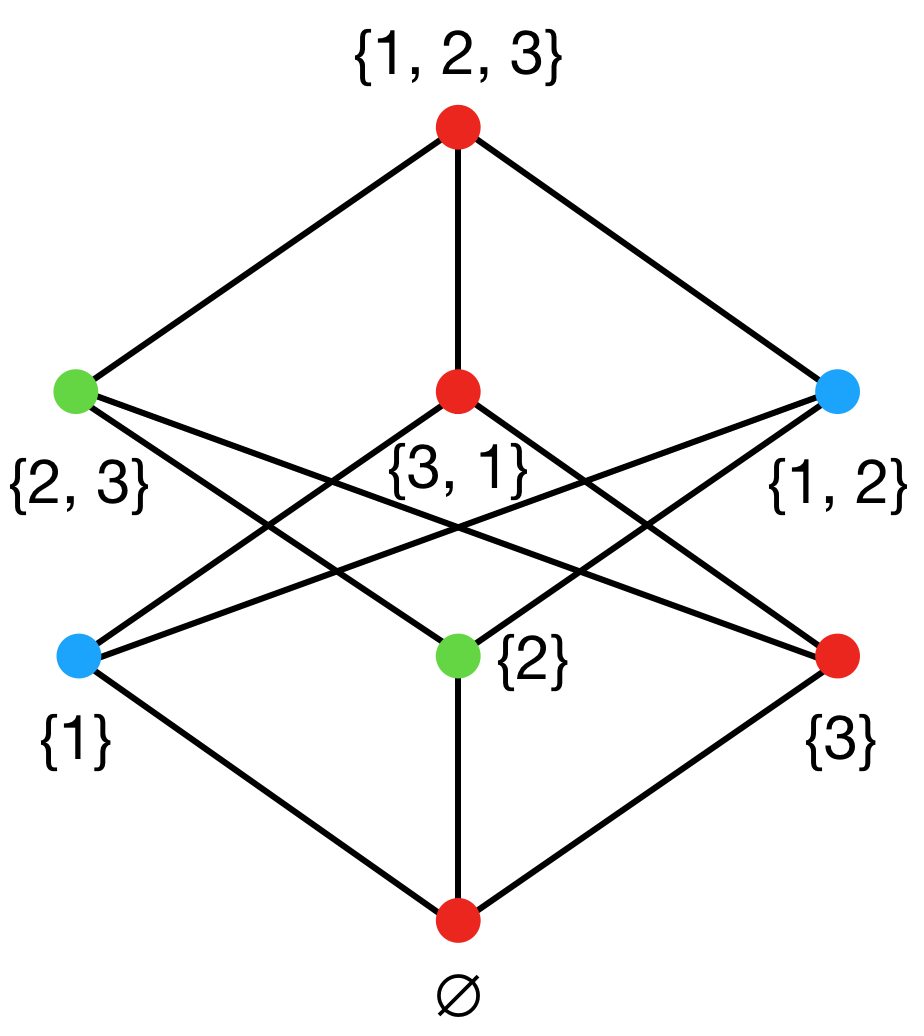
\includegraphics[scale= 0.25]{Fig01.png}
			\end{center}
		\end{figure}
	\end{example}
	
	\begin{definition}
		A set family $\mathcal{F}$ is called a Sperner system if no set in $\mathcal{F}$ contains another.
		(i.e. $\mathcal{F}$ is an antichain in itself)
	\end{definition}
	
	\begin{theorem}(Sperner)
		Let $\mathcal{F} \subseteq 2^{[n]}$ be a Sperner system. Then, $|\mathcal{F}| \leq {n \choose \lfloor n/2 \rfloor}$.
	\end{theorem}
	
	\begin{proof}
		Since this theorem is corollary of next theorem, we omit the proof.
	\end{proof}
	
	\begin{theorem}
		If $\mathcal{F} \subseteq 2^{[n]}$ is a Sperner system, then $\sum_{A \in \mathcal{F}} 1/{n \choose |A|} \leq 1$.
	\end{theorem}

	\begin{proof}
		For each $A \in \mathcal{F}$, define $S(A) = \{ \sigma \in S_n : \sigma(\{1, 2, \cdots, |A|\}) = A \}$.
		Then, $|S(A)| = |A|!(n-|A|)!$.
		Also, for each $A \neq A^{\prime} \in \mathcal{F}$, $S(A) \cap S(A^{\prime}) = \emptyset$.
		From $\cup_{A \in \mathcal{F}} S(A) \subseteq S_n$, we obtain $\sum_{A \in \mathcal{F}} |A|! (n-|A|)! \leq n!$, which concludes the proof.
	\end{proof}
	
	\newpage
	
	\section*{Exercises}
	
	\begin{theorem*}(Hall's Marriage Theorem)
		Let $G = (L \cup R, E)$ be a bipartite graph with $|L| = |R|$.
		Define $N(X)$ as the set of neighbors of vertices in $X$.
		$G$ has a perfect matching if and only if for every $X \subseteq L$, $|N(X)| \geq |X|$.
	\end{theorem*}
	
	\begin{problem}
		Prove Hall's marriage theorem using Dilworth's theorem.
	\end{problem}
	
	\begin{problem}
		Let $(P, \leq)$ be a finite poset with $|P| = ab+1$. Then, it has either a chain of size $a+1$ or an antichain of size $b+1$.
	\end{problem}
	
	\begin{theorem*}(Erd\H{o}s-Szekeres Theorem)
		Let $s = (s_1, s_2, \cdots, s_{ab+1})$ be a sequence of distinct integers.
		Then $s$ has an increasing subsequence of length $a+1$ or a decreasing subsequence of length $b+1$.
	\end{theorem*}
	
	\begin{problem}
		Prove Erd\H{o}s-Szekeres Theorem.
	\end{problem}
	
	\begin{problem}
		There are $n$ intervals $I_1, I_2, \cdots, I_n$ on the real line.
		For every $N \in {[n] \choose k}$, there exist $i \neq j \in N$, $I_i \cap I_j \neq \emptyset$.
		Prove that there exists $S \subseteq \mathbb{R}$ such that $|S| = k-1$ where $I_i \cap S \neq \emptyset$ for every $i \in [n]$.
	\end{problem}
	
	\begin{problem}(Romania TST 2005)
		Let $n$ be a positive integer and $S$ a set of $n^2+1$ positive integers with the property that every $(n+1)$-element subset of $S$ contains two numbers one of which is divisible by the other.
		Show that $S$ contains $n+1$ different numbers $a_1, a_2, \cdots , a_{n+1}$ such that $a_i | a_{i+1}$ for each $i \in [n]$.
	\end{problem}
	
\end{document}
